% Graphic for TeX using PGF
% Title: /home/ondra/Diagram1.dia
% Creator: Dia v0.97.2
% CreationDate: Thu Aug  1 08:02:11 2013
% For: ondra
% \usepackage{tikz}
% The following commands are not supported in PSTricks at present
% We define them conditionally, so when they are implemented,
% this pgf file will use them.
\ifx\du\undefined
  \newlength{\du}
\fi
\setlength{\du}{15\unitlength}
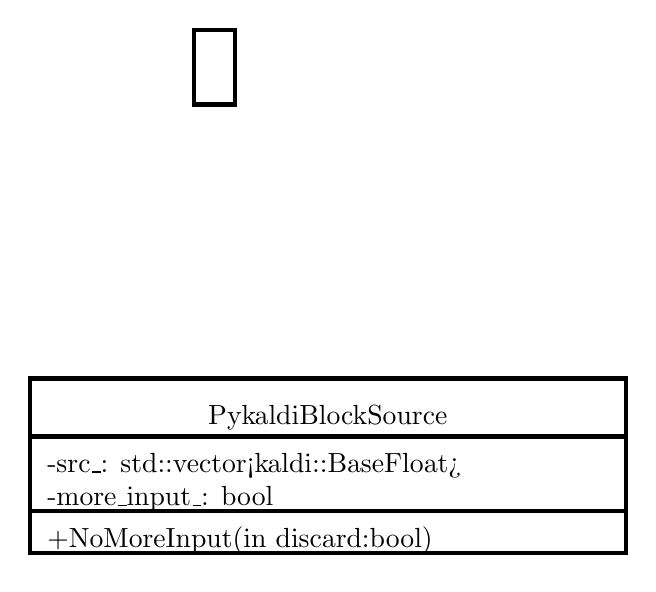
\begin{tikzpicture}
\pgftransformxscale{1.000000}
\pgftransformyscale{-1.000000}
\definecolor{dialinecolor}{rgb}{0.000000, 0.000000, 0.000000}
\pgfsetstrokecolor{dialinecolor}
\definecolor{dialinecolor}{rgb}{1.000000, 1.000000, 1.000000}
\pgfsetfillcolor{dialinecolor}
\pgfsetlinewidth{0.100000\du}
\pgfsetdash{}{0pt}
\definecolor{dialinecolor}{rgb}{1.000000, 1.000000, 1.000000}
\pgfsetfillcolor{dialinecolor}
\fill (13.250000\du,6.900000\du)--(13.250000\du,8.700000\du)--(14.250000\du,8.700000\du)--(14.250000\du,6.900000\du)--cycle;
\definecolor{dialinecolor}{rgb}{0.000000, 0.000000, 0.000000}
\pgfsetstrokecolor{dialinecolor}
\draw (13.250000\du,6.900000\du)--(13.250000\du,8.700000\du)--(14.250000\du,8.700000\du)--(14.250000\du,6.900000\du)--cycle;
% setfont left to latex
\definecolor{dialinecolor}{rgb}{0.000000, 0.000000, 0.000000}
\pgfsetstrokecolor{dialinecolor}
\node at (13.750000\du,7.995000\du){};
% setfont left to latex
\pgfsetlinewidth{0.050000\du}
\definecolor{dialinecolor}{rgb}{0.000000, 0.000000, 0.000000}
\pgfsetstrokecolor{dialinecolor}
\draw (13.750000\du,8.147500\du)--(13.750000\du,8.147500\du);
\pgfsetlinewidth{0.100000\du}
\pgfsetdash{}{0pt}
\definecolor{dialinecolor}{rgb}{1.000000, 1.000000, 1.000000}
\pgfsetfillcolor{dialinecolor}
\fill (9.300000\du,15.300000\du)--(9.300000\du,16.700000\du)--(23.660000\du,16.700000\du)--(23.660000\du,15.300000\du)--cycle;
\definecolor{dialinecolor}{rgb}{0.000000, 0.000000, 0.000000}
\pgfsetstrokecolor{dialinecolor}
\draw (9.300000\du,15.300000\du)--(9.300000\du,16.700000\du)--(23.660000\du,16.700000\du)--(23.660000\du,15.300000\du)--cycle;
% setfont left to latex
\definecolor{dialinecolor}{rgb}{0.000000, 0.000000, 0.000000}
\pgfsetstrokecolor{dialinecolor}
\node at (16.480000\du,16.250000\du){PykaldiBlockSource};
\definecolor{dialinecolor}{rgb}{1.000000, 1.000000, 1.000000}
\pgfsetfillcolor{dialinecolor}
\fill (9.300000\du,16.700000\du)--(9.300000\du,18.500000\du)--(23.660000\du,18.500000\du)--(23.660000\du,16.700000\du)--cycle;
\definecolor{dialinecolor}{rgb}{0.000000, 0.000000, 0.000000}
\pgfsetstrokecolor{dialinecolor}
\draw (9.300000\du,16.700000\du)--(9.300000\du,18.500000\du)--(23.660000\du,18.500000\du)--(23.660000\du,16.700000\du)--cycle;
% setfont left to latex
\definecolor{dialinecolor}{rgb}{0.000000, 0.000000, 0.000000}
\pgfsetstrokecolor{dialinecolor}
\node[anchor=west] at (9.450000\du,17.400000\du){-src\_: std::vector<kaldi::BaseFloat>};
% setfont left to latex
\definecolor{dialinecolor}{rgb}{0.000000, 0.000000, 0.000000}
\pgfsetstrokecolor{dialinecolor}
\node[anchor=west] at (9.450000\du,18.200000\du){-more\_input\_: bool};
\definecolor{dialinecolor}{rgb}{1.000000, 1.000000, 1.000000}
\pgfsetfillcolor{dialinecolor}
\fill (9.300000\du,18.500000\du)--(9.300000\du,19.500000\du)--(23.660000\du,19.500000\du)--(23.660000\du,18.500000\du)--cycle;
\definecolor{dialinecolor}{rgb}{0.000000, 0.000000, 0.000000}
\pgfsetstrokecolor{dialinecolor}
\draw (9.300000\du,18.500000\du)--(9.300000\du,19.500000\du)--(23.660000\du,19.500000\du)--(23.660000\du,18.500000\du)--cycle;
% setfont left to latex
\definecolor{dialinecolor}{rgb}{0.000000, 0.000000, 0.000000}
\pgfsetstrokecolor{dialinecolor}
\node[anchor=west] at (9.450000\du,19.200000\du){+NoMoreInput(in discard:bool)};
\end{tikzpicture}
